\section{Hasil dan Pembahasan}

\subsection{Gambaran Data}

\begin{figure*}[t]
\centering
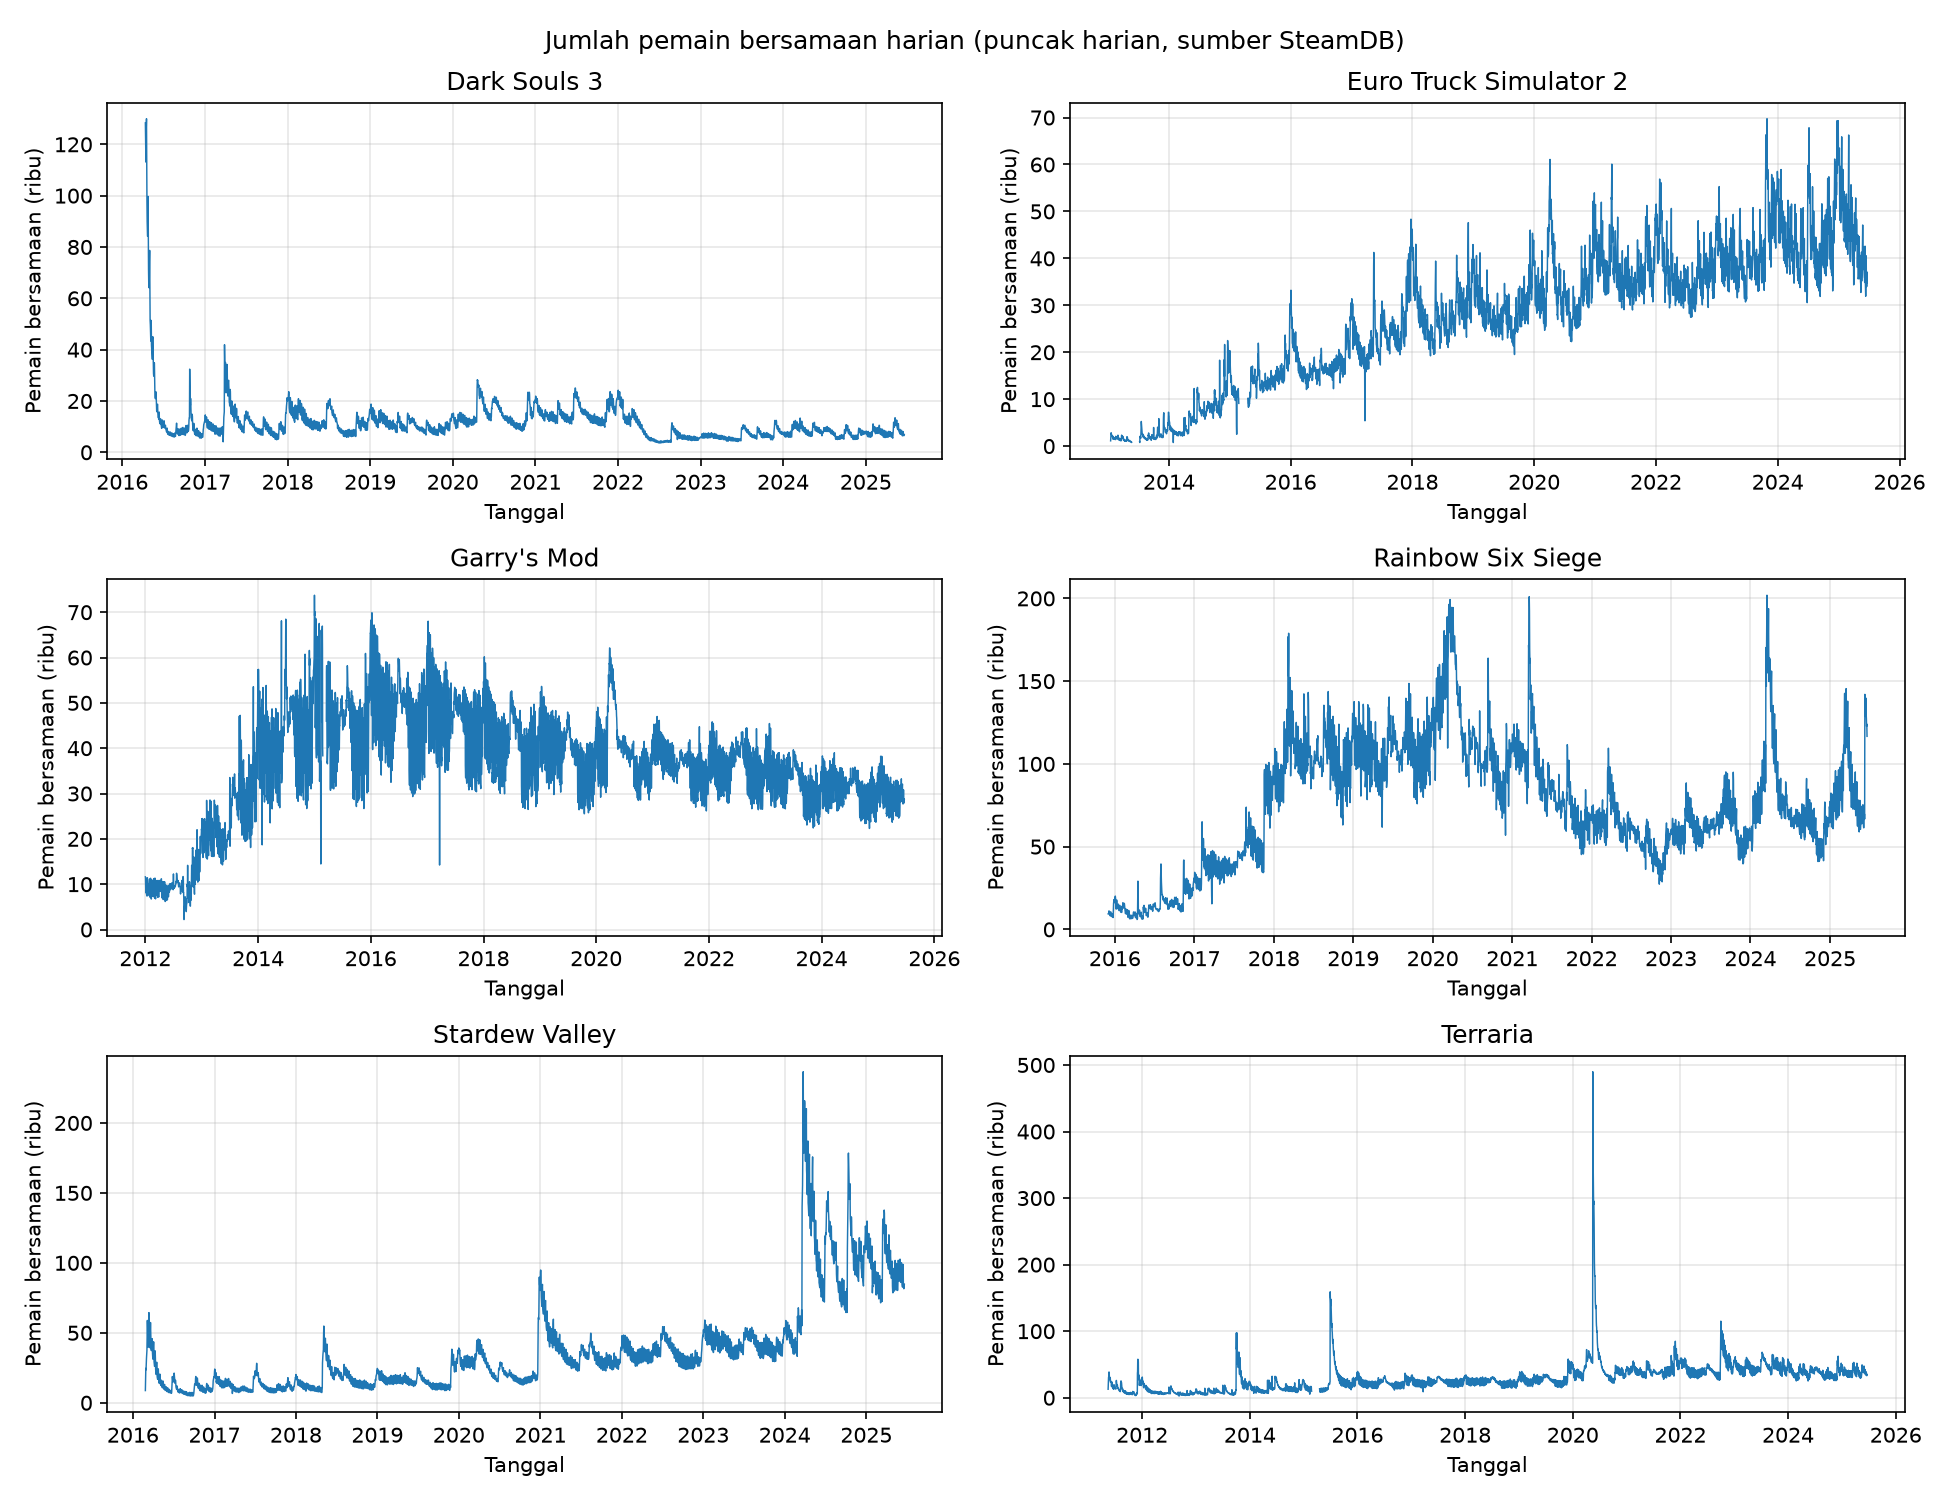
\includegraphics[width=0.58\textwidth]{01_pemain_harian.png}
\caption{Jumlah pemain bersamaan harian keenam game setelah pembersihan (sumber data: SteamDB~\cite{steamdb}).}
\label{fig:harian}
\end{figure*}

Gambar~\ref{fig:harian} memperlihatkan bahwa setiap game memiliki pola jangka panjang yang berbeda. Dark Souls 3 mencapai puncak pada awal rilis lalu turun dan stabil, ETS2 tumbuh hampir terus-menerus, sedangkan Rainbow Six Siege dan Stardew Valley naik turun dengan beberapa lonjakan besar. Terraria memiliki beberapa lonjakan yang sangat tinggi dibanding tingkat normalnya. Lonjakan seperti ini kemungkinan berkaitan dengan pembaruan besar atau event tertentu, namun penyebabnya tidak diverifikasi dalam penelitian ini.

Lonjakan alami juga terlihat pada tingkat segmen. Sebanyak 125 dari 1.229 segmen normal (10,2\%) sudah memuat satu hari dengan jumlah pemain lebih dari 1,5 kali median segmennya. Persentase tertinggi ada pada Terraria (20,1\%) dan terendah pada Rainbow Six Siege (5,2\%). Segmen-segmen ini tetap diperlakukan sebagai segmen normal.

\begin{figure}[t]
\centering
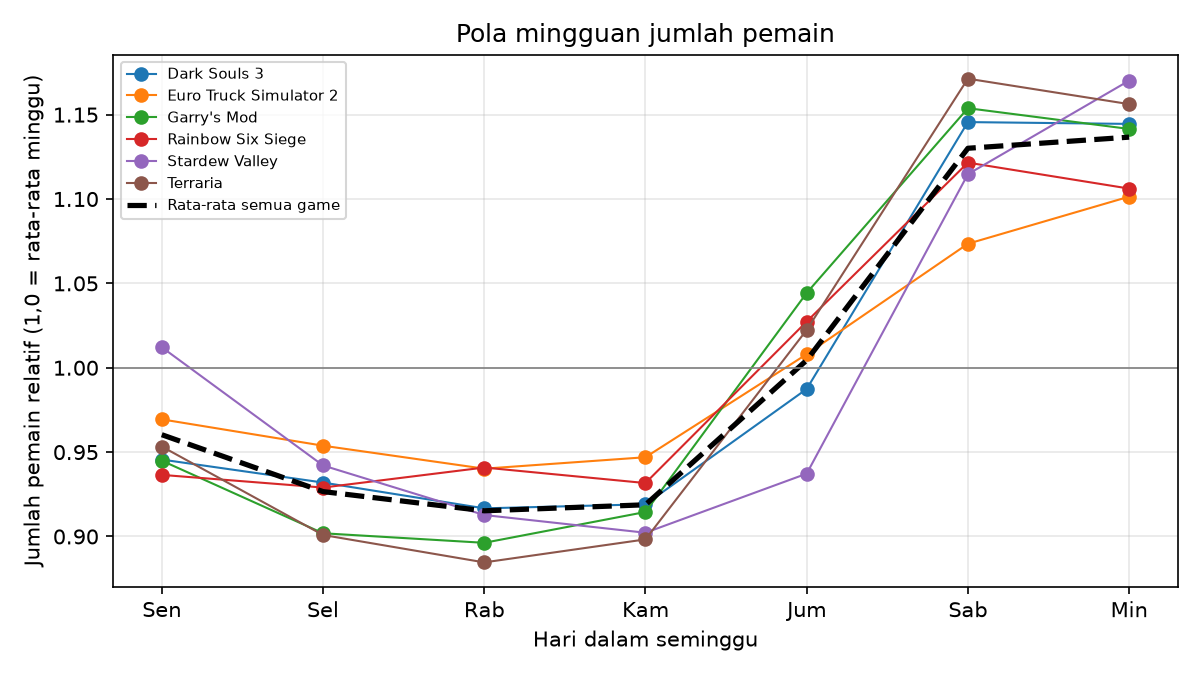
\includegraphics[width=0.92\columnwidth]{03_pola_mingguan.png}
\caption{Rata-rata jumlah pemain relatif per hari dalam seminggu. Nilai 1,0 berarti sama dengan rata-rata tujuh hari di sekitarnya.}
\label{fig:mingguan}
\end{figure}

Gambar~\ref{fig:mingguan} menunjukkan pola mingguan. Untuk menghilangkan pengaruh tren, jumlah pemain setiap hari dibagi dengan rata-rata tujuh hari di sekitarnya. Rata-rata keenam game mencapai 1,130 pada hari Sabtu dan 1,137 pada hari Minggu, sedangkan titik terendah ada pada hari Rabu (0,915). Pada setiap game, nilai Sabtu dan Minggu lebih tinggi daripada semua hari kerja.

\subsection{Hasil Encoding}

\begin{figure*}[t]
\centering
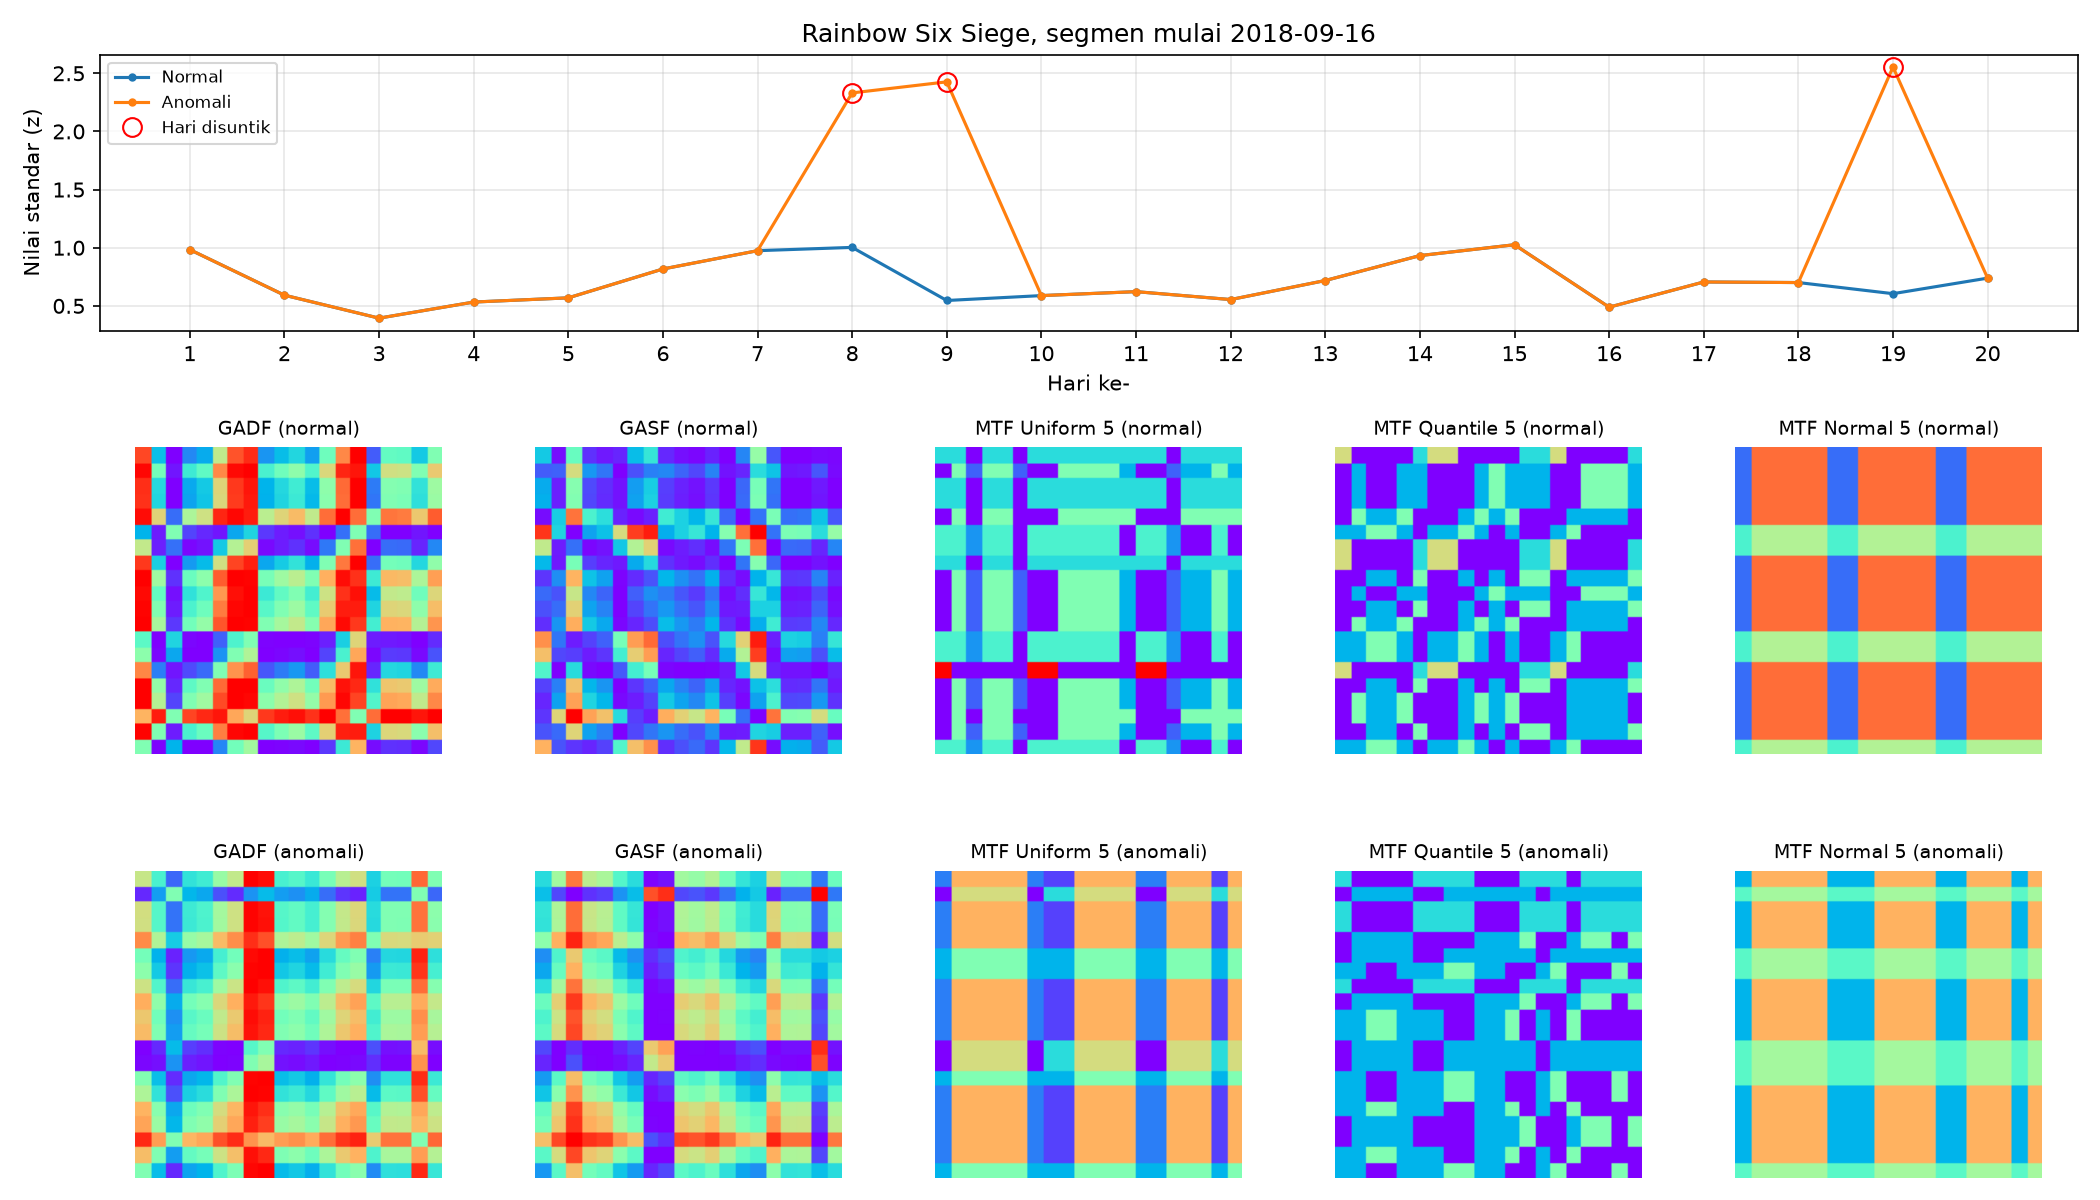
\includegraphics[width=0.66\textwidth]{05_pasangan_gambar_2.png}
\caption{Contoh segmen Rainbow Six Siege. Atas: deret waktu terstandar, dengan hari yang disuntik ditandai lingkaran merah. Tengah dan bawah: gambar dari segmen normal dan segmen anomali untuk lima encoding.}
\label{fig:pasangan}
\end{figure*}

Gambar~\ref{fig:pasangan} membandingkan gambar normal dan anomali untuk satu segmen. Pada GADF dan GASF, setiap hari yang disuntik menghasilkan garis tebal yang memotong gambar secara horizontal dan vertikal. Pada MTF Uniform, warna dominan gambar berubah. Sebaliknya, gambar MTF Quantile normal dan anomali terlihat mirip, karena pembagian bin pada strategi ini hanya bergantung pada urutan nilai dalam segmen, bukan pada besarnya.

\begin{table}[t]
\centering
\caption{Selisih statistik matriks antara data normal dan anomali}
\label{tab:delta}
\footnotesize
\begin{tabular}{lrrr}
\toprule
Encoding & \dmean & \dsd & \dcount \\
\midrule
GADF & 0,000 & 0,155 & 1,632 \\
GASF & 0,040 & 0,063 & 0,217 \\
MTF Uniform 2 & 0,165 & 0,036 & 0,015 \\
MTF Uniform 4 & 0,241 & 0,022 & 1,141 \\
MTF Uniform 5 & 0,268 & 0,033 & 1,149 \\
MTF Uniform 10 & 0,199 & 0,038 & 0,601 \\
MTF Quantile 2 & 0,000 & 0,061 & 0,124 \\
MTF Quantile 4 & 0,000 & 0,022 & 0,149 \\
MTF Quantile 5 & 0,000 & 0,014 & 0,211 \\
MTF Quantile 10 & 0,000 & 0,001 & 0,006 \\
MTF Normal 2 & 0,087 & 0,099 & 1,390 \\
MTF Normal 4 & 0,121 & 0,068 & 2,023 \\
MTF Normal 5 & 0,123 & 0,054 & 1,888 \\
MTF Normal 10 & 0,099 & 0,026 & 0,925 \\
\bottomrule
\end{tabular}
\end{table}

Tabel~\ref{tab:delta} merangkum selisih statistik matriks. Nilai \dmean{} GADF selalu nol karena matriks GADF antisimetris, dan \dmean{} MTF Quantile juga nol karena setiap bin selalu terisi sama banyak. Nilai \dcount{} pada GAF sangat kecil karena jumlah nilai unik pada matriks GADF dan GASF hampir selalu mendekati batas maksimumnya, baik untuk segmen normal maupun anomali (rata-rata 359,5 dan 361,1 untuk GADF, serta 208,3 dan 208,5 untuk GASF). Hal ini terjadi karena jumlah pemain harian hampir tidak pernah bernilai sama pada dua hari yang berbeda.

\begin{figure}[t]
\centering
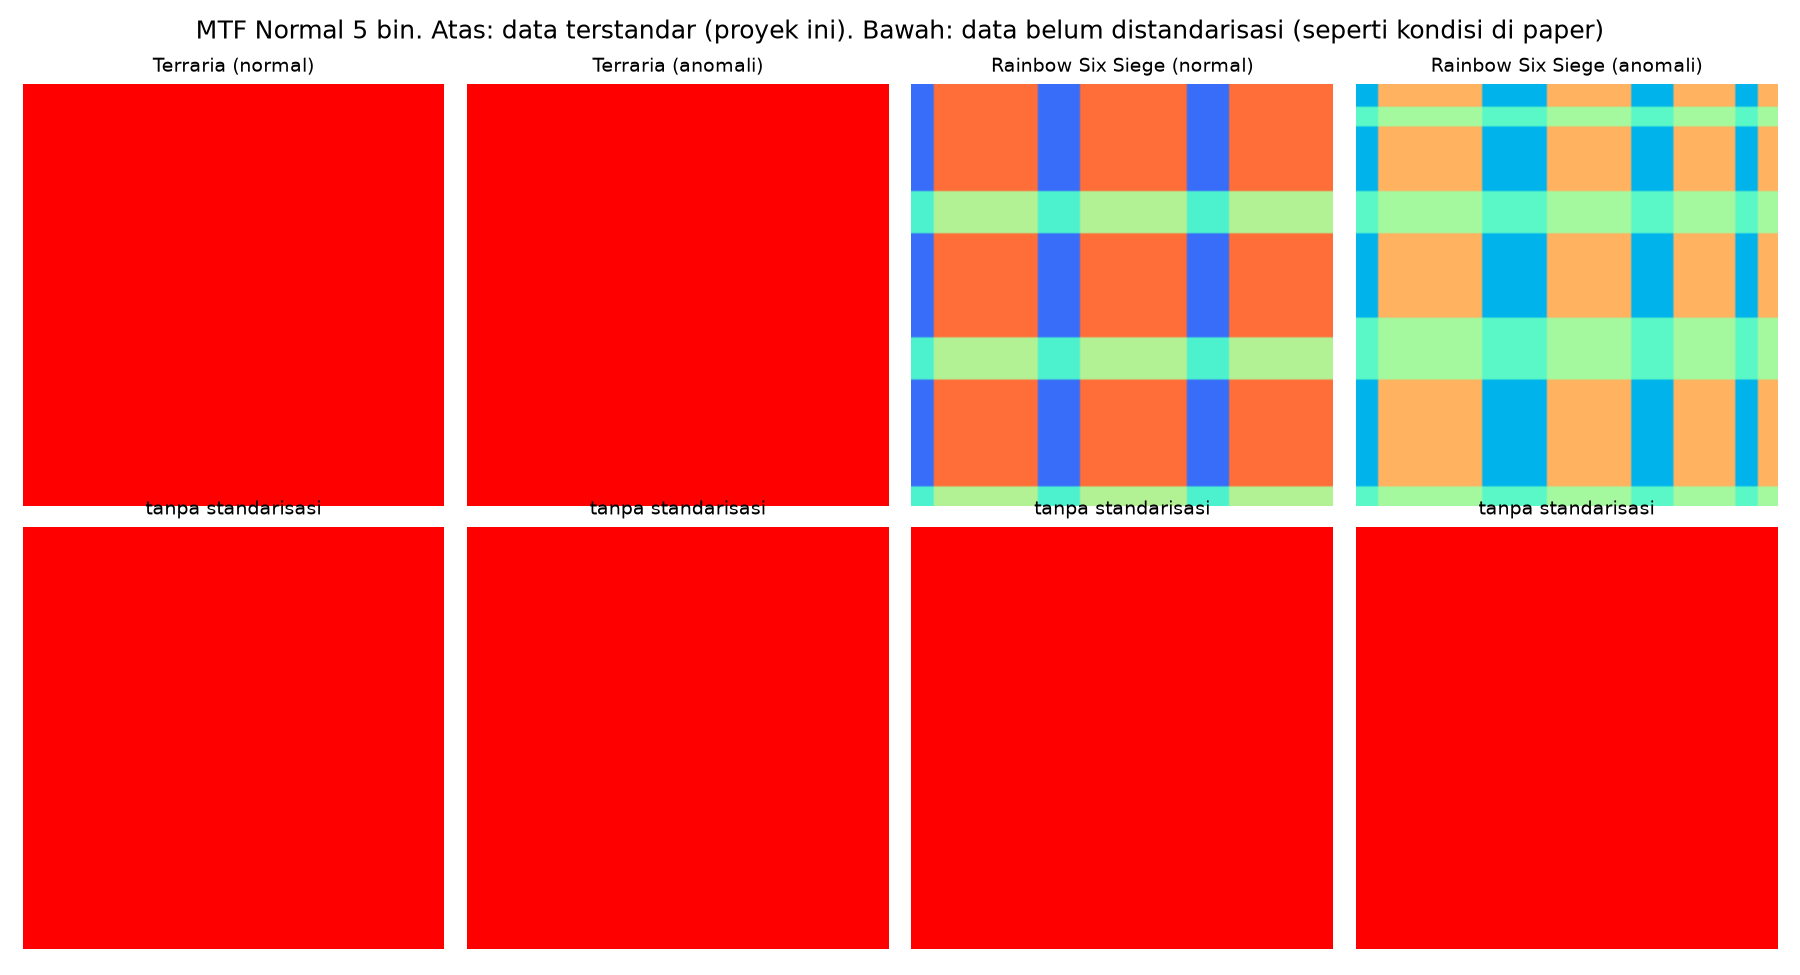
\includegraphics[width=0.9\columnwidth]{08_mtf_normal_standar_vs_mentah.png}
\caption{MTF Normal 5 bin. Atas: data terstandar seperti pada penelitian ini. Bawah: data yang belum distandarisasi, dengan seluruh gambar berwarna merah polos.}
\label{fig:mtfnormal}
\end{figure}

Hasil MTF Normal berbeda dari paper acuan, yang melaporkan bahwa seluruh gambar MTF Normal berwarna merah polos~\cite{rahadian2023}. Pada pustaka pyts, strategi normal memakai batas bin tetap dari distribusi normal baku tanpa menyesuaikan skala data. Jika semua nilai satu segmen jatuh ke bin yang sama, matriks hanya berisi angka 1 dan gambarnya menjadi merah polos. Karena data penelitian ini sudah distandarisasi, nilainya tersebar di sekitar nol sehingga melewati beberapa bin. Gambar~\ref{fig:mtfnormal} memperlihatkan perbedaan ini. Ketika MTF Normal diterapkan pada data yang hanya diubah ke $\log_{10}$ tanpa standarisasi, 100\% gambar menjadi seragam. Pada data terstandar, gambar seragam masih muncul, tetapi jauh lebih sering pada segmen normal daripada segmen anomali: 66,8\% berbanding 19,0\% untuk 2 bin, dan 8,5\% berbanding 2,5\% untuk 10 bin.

\begin{figure*}[t]
\centering
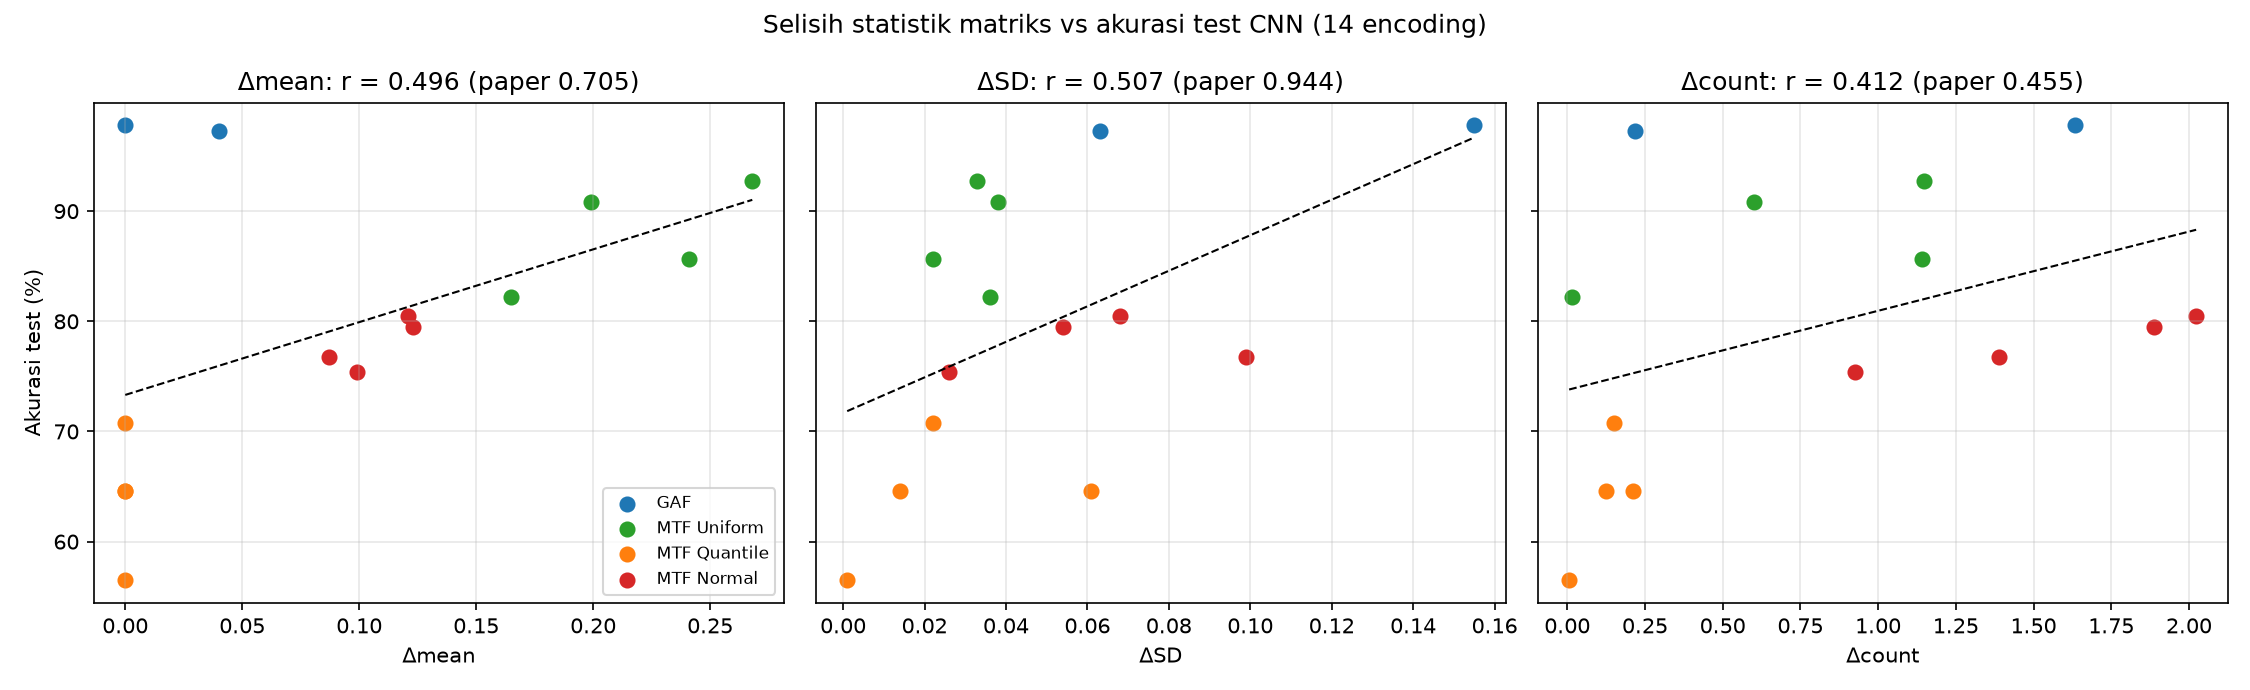
\includegraphics[width=0.82\textwidth]{12_korelasi_scatter.png}
\caption{Hubungan antara selisih statistik matriks dan akurasi test untuk 14 encoding. Garis putus-putus adalah garis regresi linear.}
\label{fig:scatter}
\end{figure*}

\subsection{Akurasi CNN}

\begin{table}[t]
\centering
\caption{Akurasi (\%) dan metrik data test untuk setiap encoding}
\label{tab:akurasi}
\footnotesize
\setlength{\tabcolsep}{3.5pt}
\begin{tabular}{lrrrrrr}
\toprule
Encoding & Train & Val & Test & Prec. & Recall & F1 \\
\midrule
GADF & 100,0 & 97,3 & 97,8 & 0,973 & 0,984 & 0,978 \\
GASF & 100,0 & 97,6 & 97,3 & 0,973 & 0,973 & 0,973 \\
MTF Uniform 2 & 97,1 & 84,2 & 82,2 & 0,829 & 0,811 & 0,820 \\
MTF Uniform 4 & 99,6 & 89,4 & 85,7 & 0,827 & 0,903 & 0,863 \\
MTF Uniform 5 & 99,9 & 92,1 & 92,7 & 0,939 & 0,914 & 0,926 \\
MTF Uniform 10 & 100,0 & 91,6 & 90,8 & 0,927 & 0,886 & 0,906 \\
MTF Quantile 2 & 80,1 & 67,9 & 64,6 & 0,665 & 0,589 & 0,625 \\
MTF Quantile 4 & 96,1 & 70,4 & 70,8 & 0,723 & 0,676 & 0,698 \\
MTF Quantile 5 & 97,3 & 70,4 & 64,6 & 0,650 & 0,632 & 0,641 \\
MTF Quantile 10 & 98,5 & 57,1 & 56,5 & 0,564 & 0,573 & 0,568 \\
MTF Normal 2 & 81,6 & 77,7 & 76,8 & 0,783 & 0,741 & 0,761 \\
MTF Normal 4 & 91,1 & 83,4 & 80,5 & 0,827 & 0,773 & 0,799 \\
MTF Normal 5 & 90,9 & 80,4 & 79,5 & 0,866 & 0,697 & 0,772 \\
MTF Normal 10 & 96,2 & 78,5 & 75,4 & 0,730 & 0,805 & 0,766 \\
\bottomrule
\end{tabular}
\end{table}

Tabel~\ref{tab:akurasi} menunjukkan bahwa GADF dan GASF memberikan akurasi test tertinggi, yaitu 97,8\% dan 97,3\%. Dari 370 gambar test, GADF hanya salah pada 8 gambar. Urutan berikutnya adalah MTF Uniform (82,2\% sampai 92,7\%), MTF Normal (75,4\% sampai 80,5\%), dan MTF Quantile (56,5\% sampai 70,8\%). Urutan keluarga encoding ini mirip dengan paper acuan, yang juga menempatkan GAF dan MTF Uniform di atas MTF Quantile~\cite{rahadian2023}, walaupun akurasi MTF Uniform pada data kami lebih rendah.

Selisih antara akurasi train dan test menunjukkan adanya overfitting pada sebagian besar encoding MTF. Contoh paling jelas adalah MTF Quantile 10 dengan akurasi train 98,5\% tetapi akurasi test hanya 56,5\%, serta MTF Normal 10 dengan 96,2\% berbanding 75,4\%. Pada GADF dan GASF selisihnya kecil (100\% berbanding 97,8\% dan 97,3\%). Karena pengaturan CNN sengaja disamakan dengan paper acuan, tidak ada regularisasi tambahan yang diberikan.

Akurasi MTF Normal berada di atas 50\%, berbeda dengan paper acuan. Analisis per gambar memperlihatkan bahwa sebagian akurasi ini berasal dari jalan pintas. Untuk 2 bin terdapat 149 gambar seragam pada data test, 120 di antaranya berasal dari segmen normal. CNN mengklasifikasikan gambar seragam dengan akurasi 80,5\%, yang sama dengan proporsi segmen normal di antara gambar seragam tersebut. Artinya, CNN menebak ``normal'' untuk setiap gambar merah polos. Pola yang sama terlihat untuk 4, 5, dan 10 bin. Pada gambar yang tidak seragam, akurasinya 74,2\% sampai 79,4\%.

Dari sisi waktu, training memerlukan rata-rata 41,2 detik per encoding, sedangkan pembuatan matriks dan gambar untuk 2.458 segmen kurang dari 0,25 detik. Seperti pada paper acuan~\cite{rahadian2023}, training CNN adalah bagian yang paling memakan waktu.

\begin{figure*}[t]
\centering
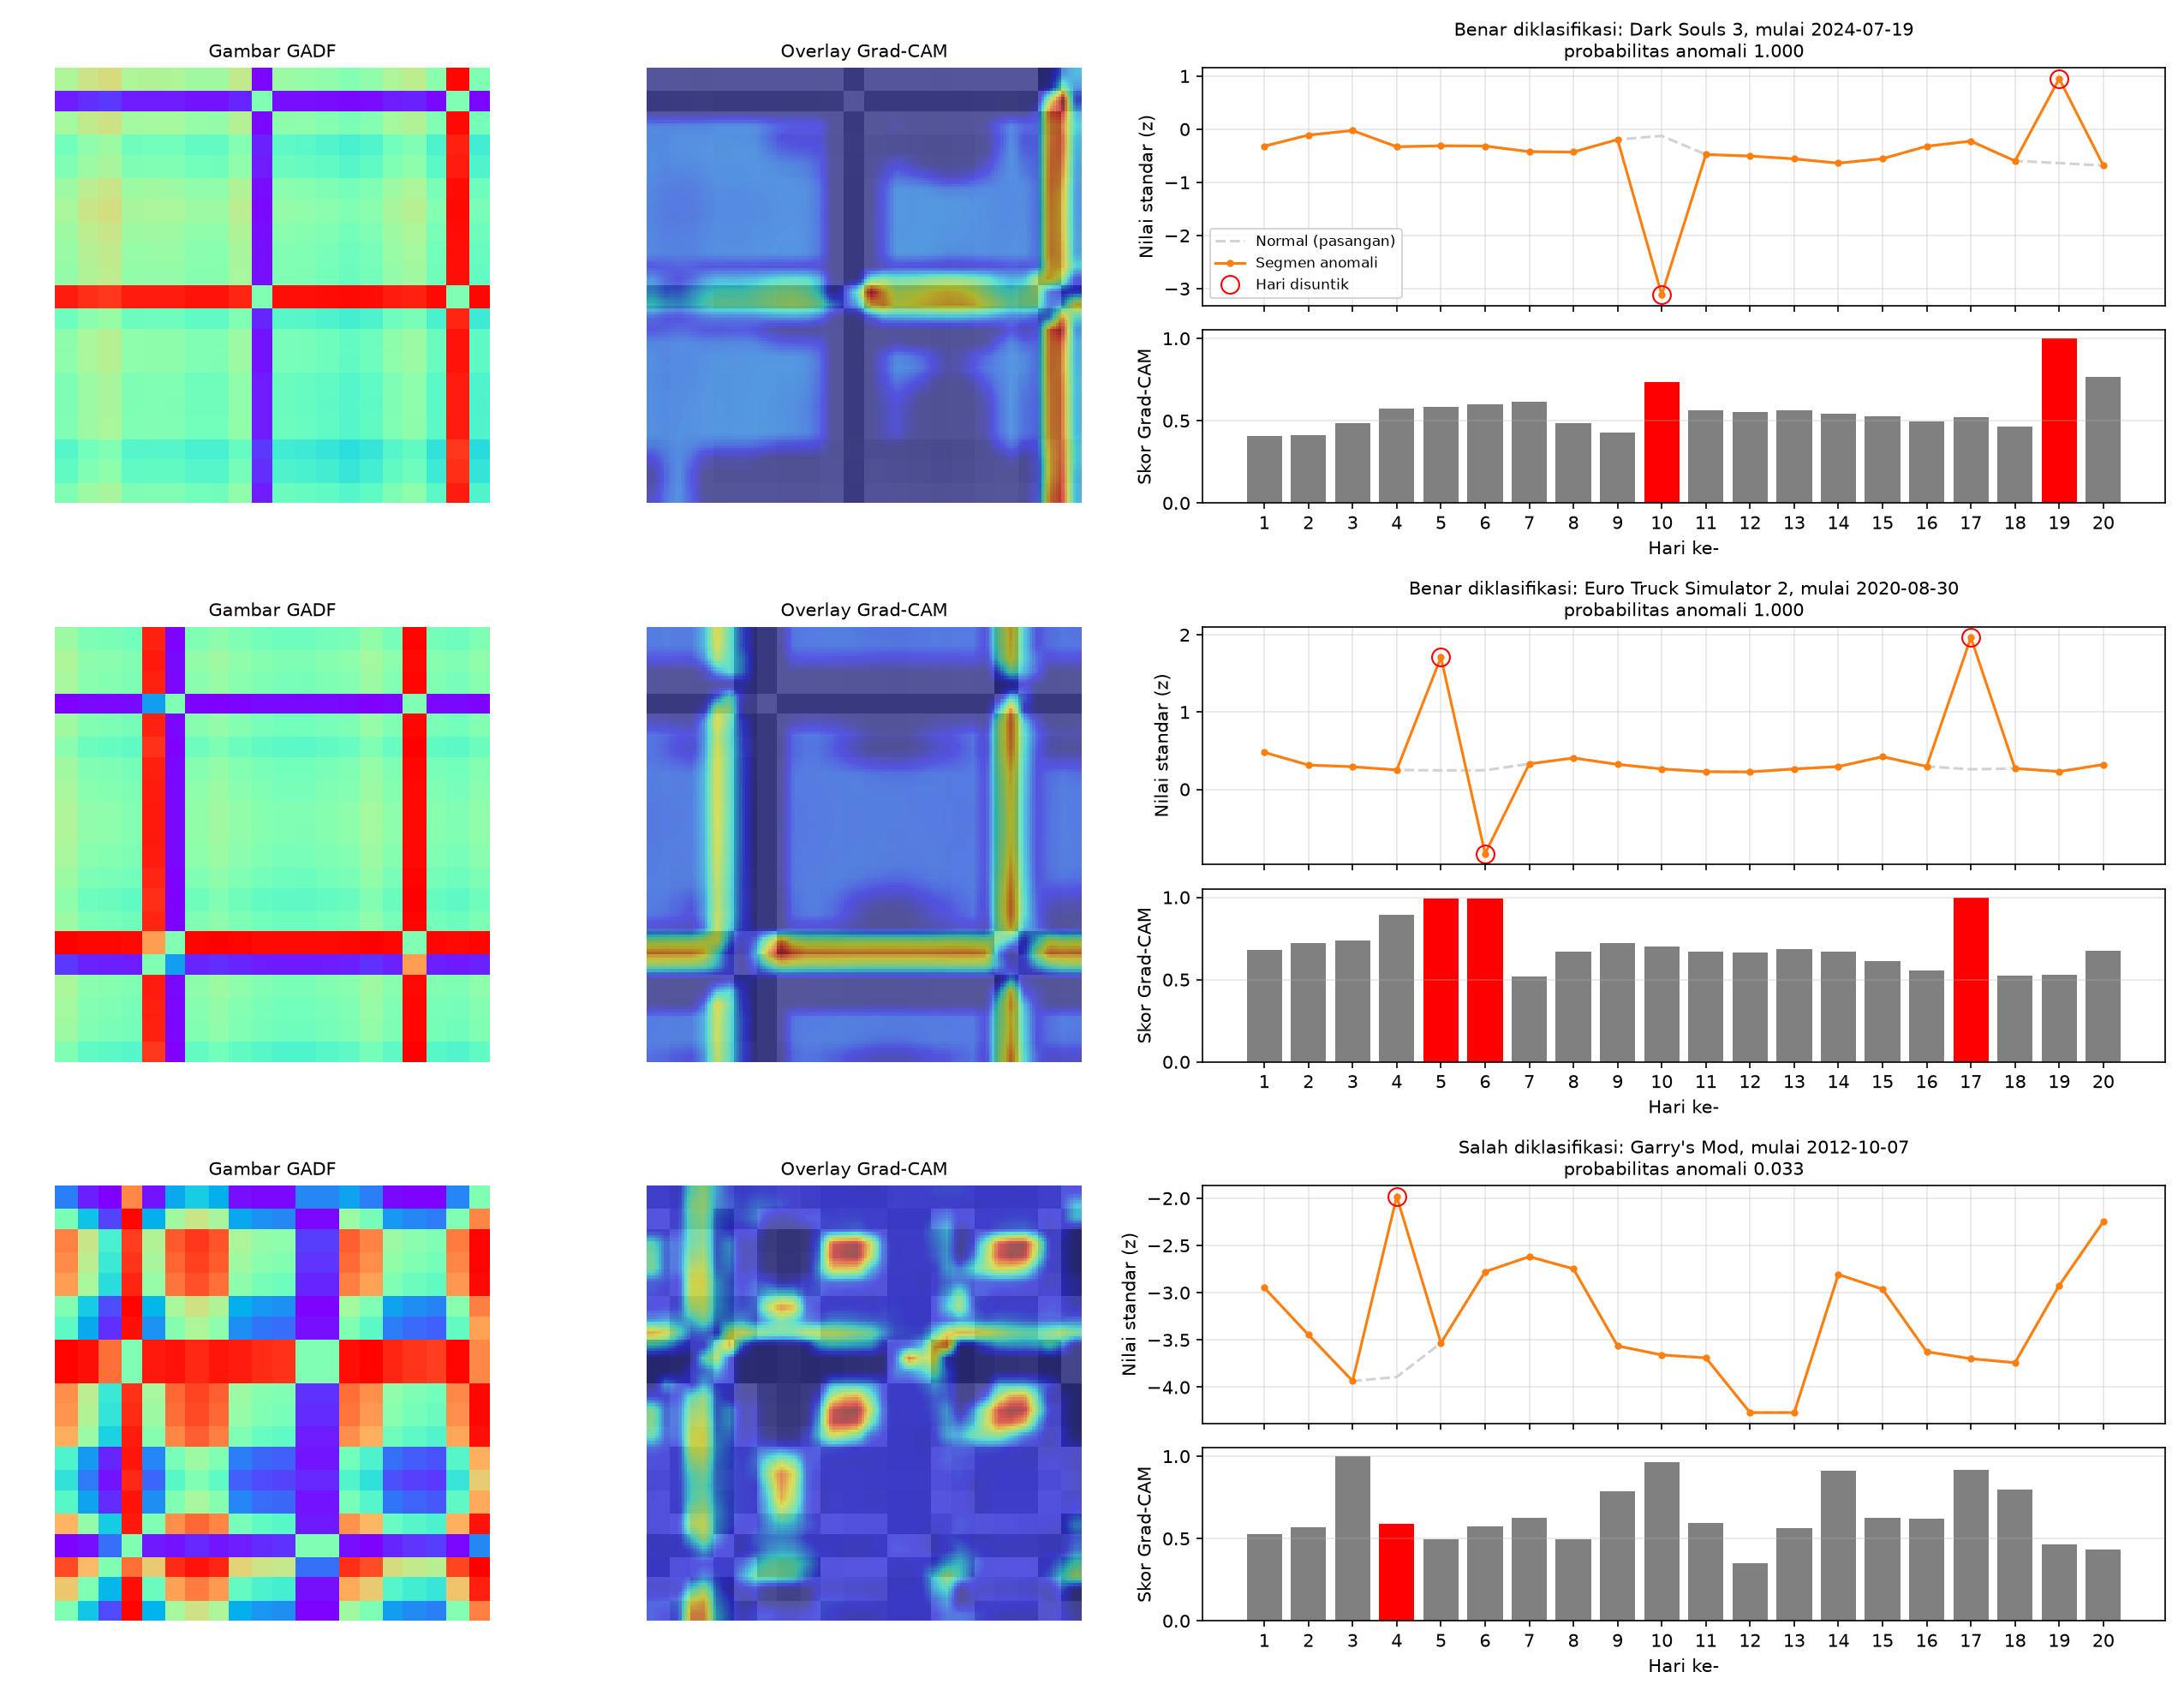
\includegraphics[width=0.6\textwidth]{13_gradcam_contoh.png}
\caption{Grad-CAM pada model GADF untuk tiga segmen anomali dari data test. Kolom kiri ke kanan: gambar GADF, overlay Grad-CAM, deret waktu (lingkaran merah menandai hari yang disuntik), dan skor Grad-CAM per hari (batang merah adalah hari yang disuntik).}
\label{fig:gradcam}
\end{figure*}

\subsection{Korelasi Pearson}

\begin{table}[t]
\centering
\caption{Korelasi Pearson antara selisih statistik dan akurasi test}
\label{tab:korelasi}
\begin{tabular}{lrr}
\toprule
Fitur & $r$ penelitian ini & $r$ paper acuan~\cite{rahadian2023} \\
\midrule
\dmean & 0,496 & 0,705 \\
\dsd & 0,507 & 0,944 \\
\dcount & 0,412 & 0,455 \\
\bottomrule
\end{tabular}
\end{table}

Tabel~\ref{tab:korelasi} dan Gambar~\ref{fig:scatter} membandingkan korelasi pada data ini dengan paper acuan. Urutan nilainya sama, yaitu \dsd{} tertinggi diikuti \dmean{} dan \dcount, tetapi kekuatannya berbeda. Nilai \dsd{} (0,507) dan \dmean{} (0,496) hampir sama, dan dengan hanya 14 titik selisih sekecil itu tidak dapat dianggap bermakna. Korelasi \dsd{} juga jauh lebih lemah daripada 0,944 pada paper acuan.

Ada beberapa kemungkinan penyebab perbedaan ini. Pertama, MTF Uniform mencapai akurasi 82,2\% sampai 92,7\% walaupun nilai \dsd-nya hanya 0,022 sampai 0,038. Kekuatan MTF Uniform pada data ini tampaknya berasal dari \dmean{} yang besar, sehingga titik-titiknya berada jauh di atas garis regresi \dsd. Kedua, pada paper acuan keempat varian MTF Normal memiliki semua selisih bernilai nol dengan akurasi 50\%~\cite{rahadian2023}. Kelompok titik ini kemungkinan ikut memperkuat korelasi. Pada data kami MTF Normal tidak berada di titik tersebut, sehingga pola yang rapi itu tidak muncul. Ketiga, \dmean{} bernilai nol untuk encoding terbaik (GADF) maupun terburuk (MTF Quantile), sehingga \dmean{} tidak dapat membedakan keduanya. Keempat, \dcount{} pada GAF hampir konstan seperti dijelaskan sebelumnya. Hanya \dcount{} yang korelasinya mendekati paper acuan (0,412 berbanding 0,455).

\subsection{Grad-CAM}

Grad-CAM diterapkan pada model GADF karena akurasi test-nya tertinggi. Dari 185 segmen anomali pada data test, model ini mengklasifikasikan 182 segmen dengan benar. Gambar~\ref{fig:gradcam} menampilkan dua contoh yang benar dan satu contoh yang salah, dipilih secara acak dengan seed tetap. Pada contoh ETS2 (segmen mulai 30 Agustus 2020), tiga hari dengan skor Grad-CAM tertinggi adalah hari ke-5, 6, dan 17, sama persis dengan tiga hari yang disuntik. Pada contoh Dark Souls 3 (mulai 19 Juli 2024), hari yang disuntik adalah hari ke-10 dan 19, sedangkan dua skor tertinggi jatuh pada hari ke-19 dan 20. Hari ke-20 kemungkinan ikut terang karena bertetangga dengan hari ke-19 dan peta Grad-CAM memiliki resolusi yang lebih rendah daripada gambar. Pada kedua contoh ini, area yang disorot adalah garis silang pada gambar GADF yang bersesuaian dengan hari anomali.

Contoh yang salah berasal dari Garry's Mod (mulai 7 Oktober 2012). Hari yang disuntik hanya hari ke-4, dan model memberikan probabilitas anomali 0,033. Peta Grad-CAM-nya tersebar ke banyak area dan skor tertinggi jatuh pada hari ke-3. Deret waktu segmen ini sudah naik turun cukup besar secara alami, sehingga satu hari lonjakan buatan tidak terlihat menonjol.
